\documentclass{standalone}

%----------------------------------------------------------------------------------------------%
%                                 Packages and basic declarations
%----------------------------------------------------------------------------------------------%

\usepackage[utf8]{inputenc}
\usepackage{pgfplots}
\usepackage{tikz}


%----------------------------------------------------------------------------------------------%
%----------------------------------------------------------------------------------------------%
%                                            DOCUMENT STARTS
%----------------------------------------------------------------------------------------------%
%----------------------------------------------------------------------------------------------%

\begin{document}


%Tikz picture starts%

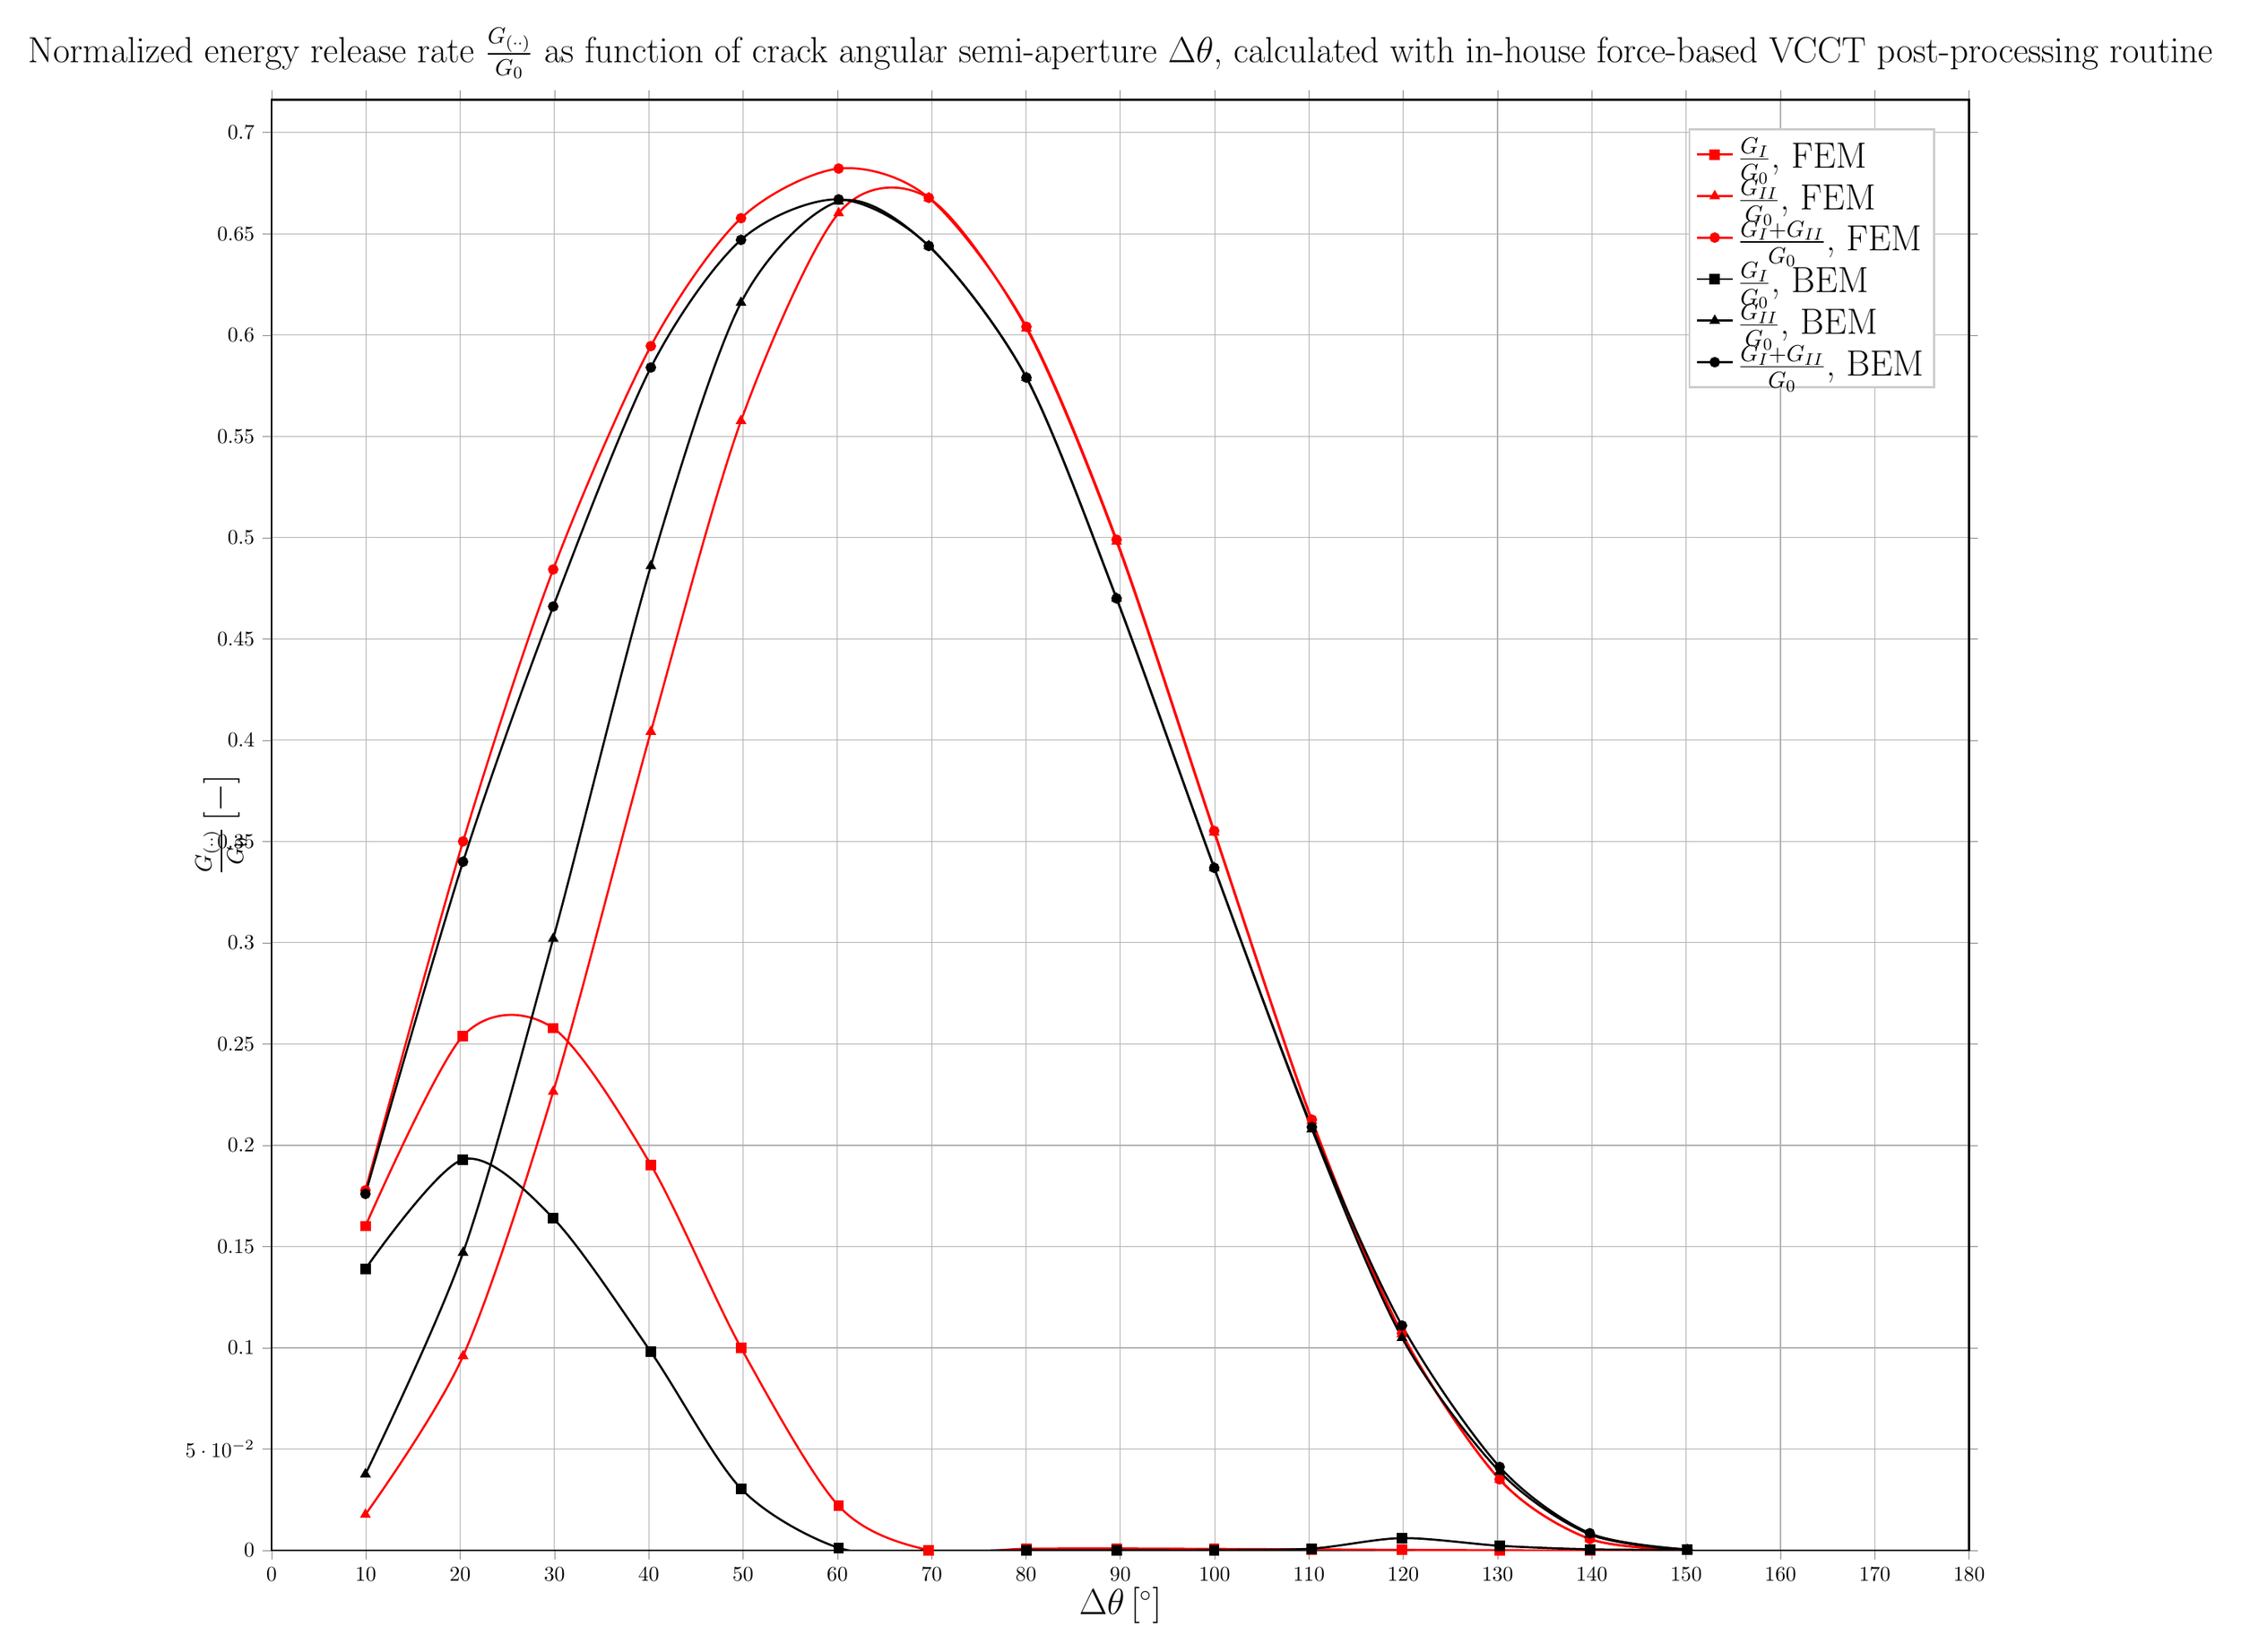
\begin{tikzpicture}

%Tikz axis starts%

\begin{axis}[width=30cm,
title={Normalized energy release rate $\frac{G_{\left(\cdot\cdot\right)}}{G_{0}}$ as function of crack angular semi-aperture  $\Delta\theta$, calculated with in-house force-based VCCT post-processing routine},
title style={font=\fontsize{16}{8}\selectfont},
xlabel style={at={(axis description cs:0.5,-0.02)},anchor=north,font=\fontsize{16}{8}\selectfont},
ylabel style={at={(axis description cs:-0.01,.5)},anchor=south,font=\fontsize{16}{8}\selectfont},
xlabel={$\Delta\theta\left[^{\circ}\right]$},ylabel={$\frac{G_{\left(\cdot\cdot\right)}}{G_{0}}\left[-\right]$},
xmin=0.0,
xmax=180.0,
ymin=0.0,
ymax=0.716322964554,
tick align=outside,
tick label style={font=\normalsize},
xtick={0.0,10.0,20.0,30.0,40.0,50.0,60.0,70.0,80.0,90.0,100.0,110.0,120.0,130.0,140.0,150.0,160.0,170.0,180.0},
xmajorgrids,
x grid style={lightgray!92.026143790849673!black},
ymajorgrids,
y grid style={lightgray!92.026143790849673!black},
line width=0.35mm,
legend style={draw=white!80.0!black,font=\fontsize{16}{12}\selectfont},
legend entries={{$\frac{G_{I}}{G_{0}}$, FEM},{$\frac{G_{II}}{G_{0}}$, FEM},{$\frac{G_{I}+G_{II}}{G_{0}}$, FEM},{$\frac{G_{I}}{G_{0}}$, BEM},{$\frac{G_{II}}{G_{0}}$, BEM},{$\frac{G_{I}+G_{II}}{G_{0}}$, BEM}},
legend cell align={left}
]

\addplot[red,smooth,mark=square*]
table{
9.95590315404 0.1600787644
20.3094667517 0.254046485477
29.8671878064 0.257843070844
40.2210818145 0.190369880501
49.7789172749 0.100059761026
60.1328146981 0.0219862407985
69.6905306301 0.000132658083889
80.044093374 0.000829962765018
89.6017683249 0.000937454428245
99.9559048047 0.000751935160957
110.309467549 0.000523666500357
119.867183481 0.000287031127092
130.221080904 0.000110964580079
139.778919779 1.83745208803e-05
150.132817203 0.000398968142875
};

\addplot[red,smooth,mark=triangle*]
table{
9.95590315404 0.0176892726033
20.3094667517 0.0959921286311
29.8671878064 0.226469539389
40.2210818145 0.404209202094
49.7789172749 0.557647807424
60.1328146981 0.660226106395
69.6905306301 0.667631671414
80.044093374 0.603290922564
89.6017683249 0.498044742797
99.9559048047 0.35445671412
110.309467549 0.212143093856
119.867183481 0.106894177549
130.221080904 0.0349524196076
139.778919779 0.00564722639295
150.132817203 0.000168821468764
};

\addplot[red,smooth,mark=*]
table{
9.95590315404 0.177768037003
20.3094667517 0.350038614108
29.8671878064 0.484312610233
40.2210818145 0.594579082594
49.7789172749 0.657707568451
60.1328146981 0.682212347194
69.6905306301 0.667764329498
80.044093374 0.604120885329
89.6017683249 0.498982197225
99.9559048047 0.355208649281
110.309467549 0.212666760356
119.867183481 0.107181208676
130.221080904 0.0350633841877
139.778919779 0.00566560091384
150.132817203 0.000567789611639
};

\addplot[black,smooth,mark=square*]
table{
9.95590315404 0.139
20.3094667517 0.193
29.8671878064 0.164
40.2210818145 0.098
49.7789172749 0.0305
60.1328146981 0.00127
69.6905306301 -4.79e-05
80.044093374 6.85e-05
89.6017683249 0.000112
99.9559048047 0.000112
110.309467549 0.000895
119.867183481 0.00607
130.221080904 0.00229
139.778919779 0.000552
150.132817203 0.000306
};

\addplot[black,smooth,mark=triangle*]
table{
9.95590315404 0.0376
20.3094667517 0.147
29.8671878064 0.302
40.2210818145 0.486
49.7789172749 0.616
60.1328146981 0.666
69.6905306301 0.644
80.044093374 0.579
89.6017683249 0.47
99.9559048047 0.337
110.309467549 0.208
119.867183481 0.105
130.221080904 0.0389
139.778919779 0.00792
150.132817203 0.000165
};

\addplot[black,smooth,mark=*]
table{
9.95590315404 0.176
20.3094667517 0.34
29.8671878064 0.466
40.2210818145 0.584
49.7789172749 0.647
60.1328146981 0.667
69.6905306301 0.644
80.044093374 0.579
89.6017683249 0.47
99.9559048047 0.337
110.309467549 0.209
119.867183481 0.111
130.221080904 0.0412
139.778919779 0.00847
150.132817203 0.000471
};

\end{axis}
%Tikz axis ends%


\end{tikzpicture}
%Tikz picture ends%


\end{document}

%----------------------------------------------------------------------------------------------%
%----------------------------------------------------------------------------------------------%
%                                            DOCUMENT ENDS
%----------------------------------------------------------------------------------------------%
%----------------------------------------------------------------------------------------------%

